

\subsection{GAPP - Screenshots}
\label{sec:gapp-screenshots}
\begin{figure}
	\begin{minipage}[b]{0.4\linewidth}
		\centering
			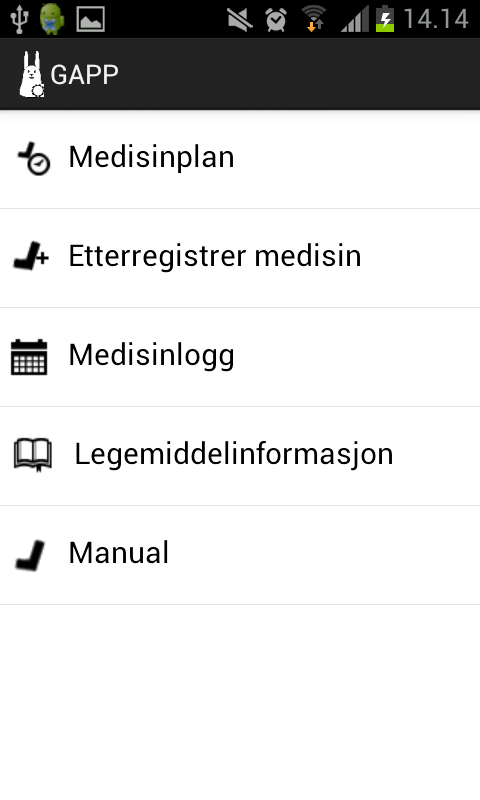
\includegraphics[width=0.20\paperwidth]{Pictures/Screenshots/gapp_main_menu.png}
		\caption{GAPP main menu}
		\label{fig:gapp-main-menu}
	\end{minipage}
	\hspace{3cm}
	\begin{minipage}[b]{0.4\linewidth}
		\centering
		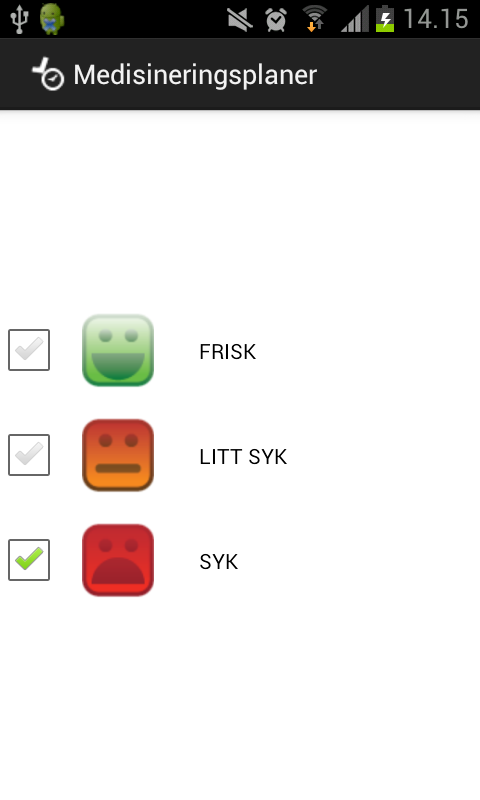
\includegraphics[width=0.20\paperwidth]{Pictures/Screenshots/gapp_view_plans.png}
	\caption{Available plans in GAPP}
	\label{fig:gapp-view-plans}
	\end{minipage}
\end{figure}

\begin{figure}
	\begin{minipage}[b]{0.4\linewidth}
		\centering
		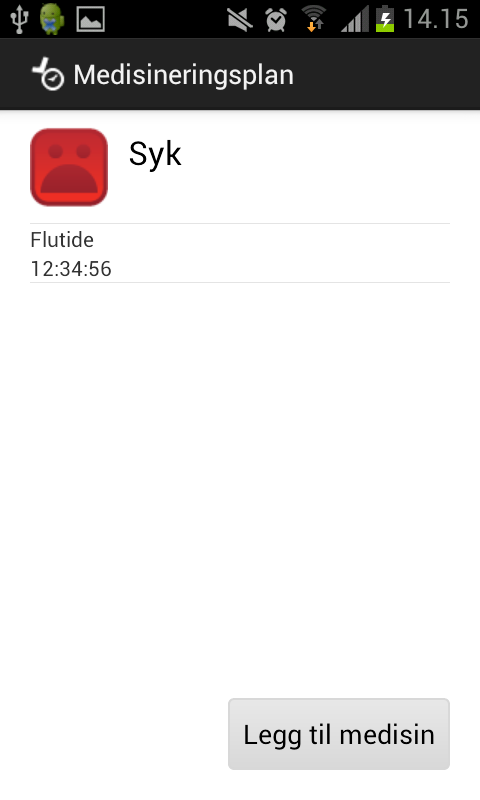
\includegraphics[width=0.20\paperwidth]{Pictures/Screenshots/gapp_plan.png}
	\caption{A medication plan in GAPP}
	\label{fig:gapp-plan}
	\end{minipage}
	\hspace{3cm}
	\begin{minipage}[b]{0.4\linewidth}
		\centering
		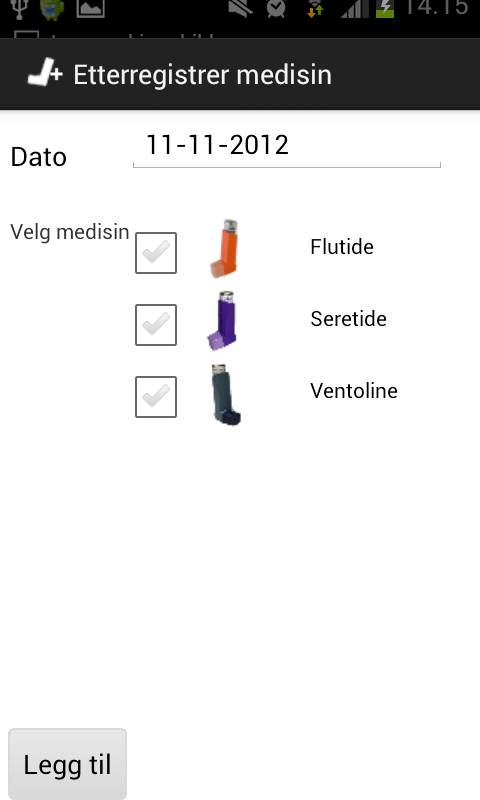
\includegraphics[width=0.20\paperwidth]{Pictures/Screenshots/register_treatment.png}
	\caption{Register treatment in GAPP}
	\label{fig:gapp-register-treatment}
	\end{minipage}
\end{figure}

\begin{figure}
	\begin{minipage}[b]{0.4\linewidth}
		\centering
		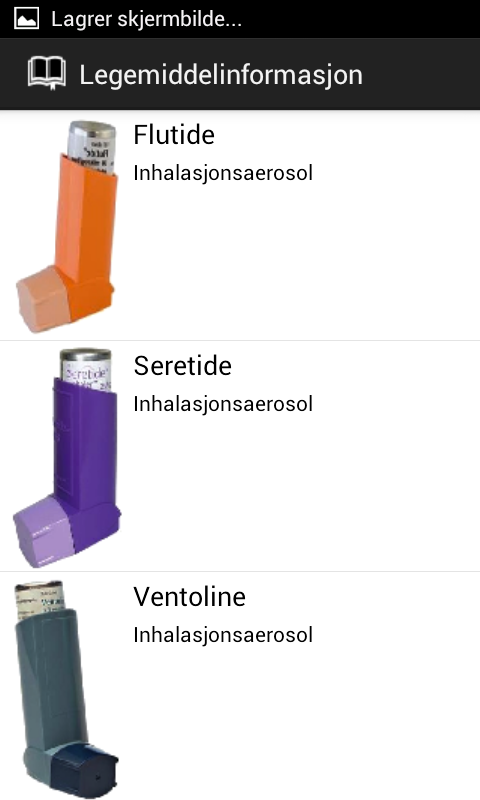
\includegraphics[width=0.20\paperwidth]{Pictures/Screenshots/information.png}
	\caption{Choose among medicines to view more information}
	\label{fig:gapp-infomration}
	\end{minipage}
	\hspace{3cm}
	\begin{minipage}[b]{0.4\linewidth}
		\centering
		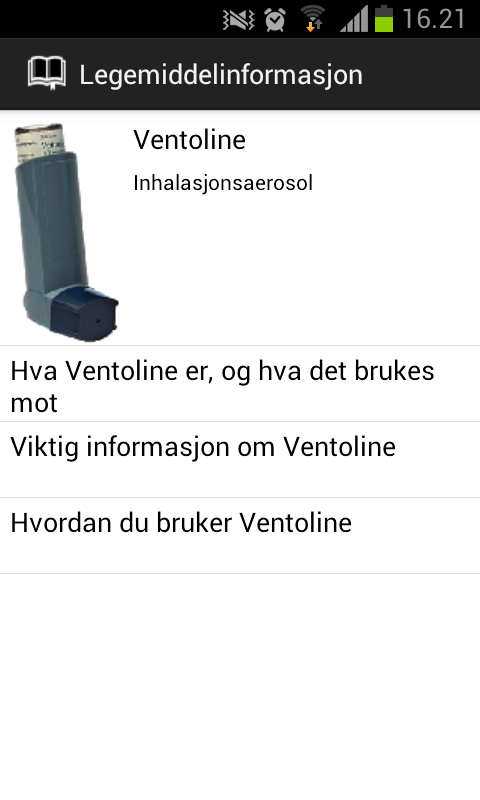
\includegraphics[width=0.20\paperwidth]{Pictures/Screenshots/specific_information.png}
	\caption{Medicine specific information}
	\label{fig:gapp-medicine-information}
	\end{minipage}
\end{figure}


\begin{figure}
	\begin{minipage}[b]{0.4\linewidth}
		\centering
		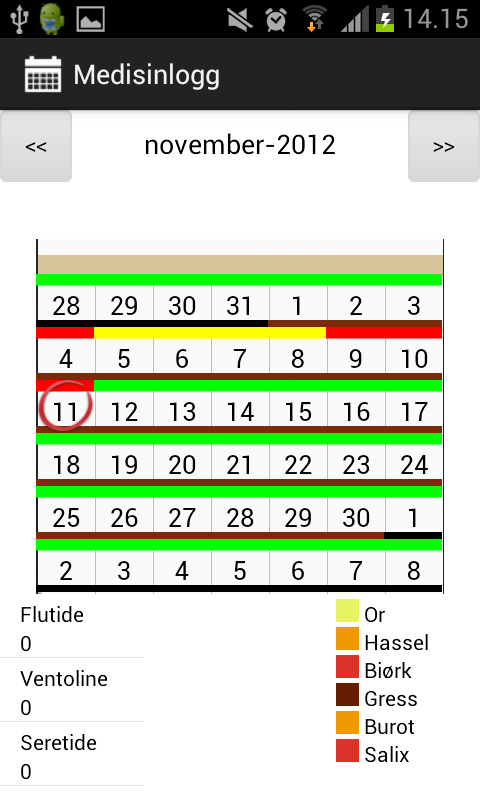
\includegraphics[width=0.20\paperwidth]{Pictures/Screenshots/logg.png}
	\caption{Medicine log in GAPP}
	\label{fig:gapp-log}
	\end{minipage}
\end{figure}




Figure \ref{fig:gapp-main-menu} shows the main menu. The item ``manual'' is a bit misguiding, as this shows an image gallery of 
how a child should take the medicine (shake, put on mask, and so on). We did not have time to make a proper manual on how to use the
application, but hopefully, the application is intuitive enough.


Figure \ref{fig:gapp-view-plans} shows the available plans for an adult. By pressing one of the checkboxes, the child's medical plan
is updated appropriatly. By touching the name of a plan, you get presented with the screen below. 

Figure \ref{fig:gapp-plan} view contains a list of the medicines that are stored in a medicine plan. You can add a medicine through the button, 
and by touching a medicine, you can delete it. 
  

Figure \ref{fig:gapp-log} shows the log of a child.
The log consists mainly of 3 components. The calendar shows the days of a month, the chosen medicine plan for a child on a
given day, indicated by a green/yellow/red line, and the distribution of pollen at that day, indicated by the bottom line of each cell. 


This pollen distribution is given by our dummy xml-feed (since pollenvarslingen.no is not currently casting). 
We have used the same distribution for each day, which explains why every day is brown. Down to the left, one can see how many
times the child has taken the given medicine at a day. Down to the right, you can see the pollen spread at the day for every type 
of pollen that is casted by pollenvarslingen.no. 
The cells of the calendar is touchable, and the listviews on the bottom of the page is updated according to which day is selected.


It is possible to register a treatment after the medication is taken. This is done by choosing the date (which is autofilled with todays date),
and choosing a medicine. The child then gets stars in his/her treasure chest. 

\subsubsection{CAPP - Screenshots}
\label{sec:capp-screenshots}
\begin{figure}
	\begin{minipage}[b]{0.4\linewidth}
		\centering
		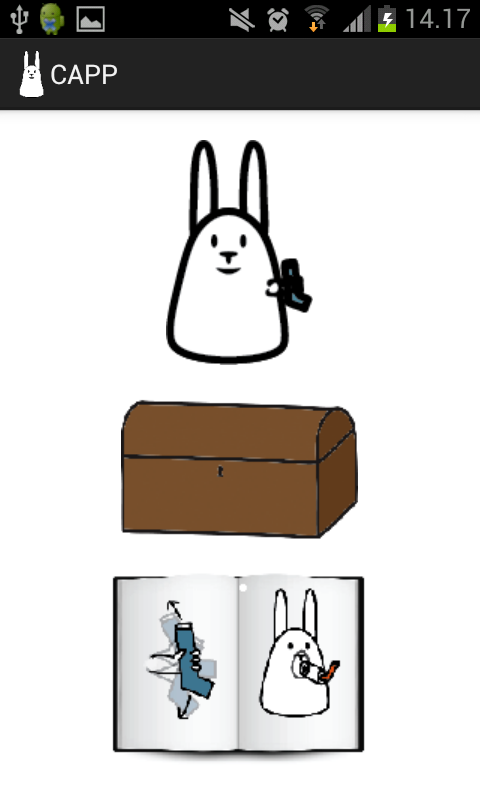
\includegraphics[width=0.20\paperwidth]{Pictures/Screenshots/capp_main_menu.png}
	\caption{Main menu in CAPP}
	\label{fig:capp-main-menu}
	\end{minipage}
	\hspace{3cm}
	\begin{minipage}[b]{0.4\linewidth}
		\centering
		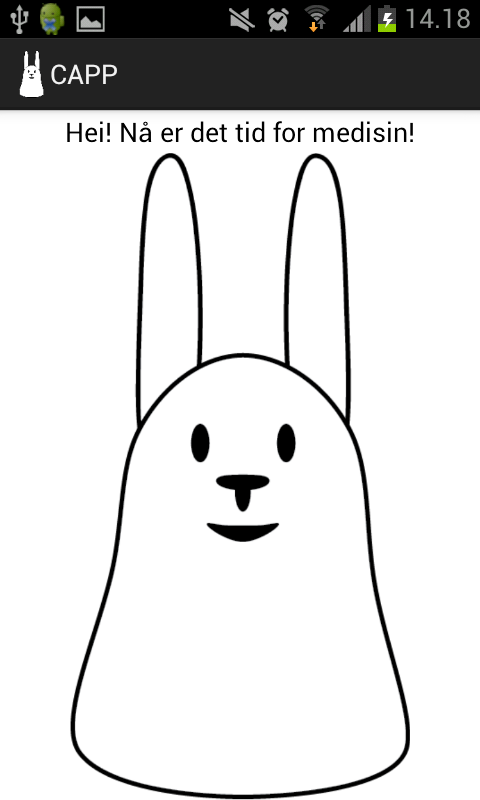
\includegraphics[width=0.20\paperwidth]{Pictures/Screenshots/capp_start_treatment.png}
	\caption{Start a treamtment in CAPP}
	\label{fig:capp-start-treatment}
	\end{minipage}
\end{figure}

\begin{figure}
	\centering
		
\includegraphics[width=0.20\paperwidth]{Pictures/Screenshots/capp_stars.png}
	\caption{Amount of stars collected in CAPP}
	\label{fig:capp-stars}
\end{figure}

Figure \ref{fig:capp-main-menu} shows the main menu of CAPP. This main menu has three items. To start a treatment, the user chooses the karotz-icon. 
To see amount of stars, the child picks the treasurechest, which leads the user to Figure \ref{fig:capp-stars} 
The book leads to a series of children-friendly images, where the child can have a look at instructions for taking a medicine.   


